\documentclass[../jarvis.tex]{subfiles}
\graphicspath{{\subfix{../images/}}}

\begin{document}
\subsection{Some Proof Techniques}
\subsubsection{Proof by Contradiction}
Our first question showcases the powerful \textit{proof by contradiction}. It is mostly used when a direct proof is less feasible, and so is an indirect approach to a problem.

The main idea is to begin with an (absurd) assumption and working towards deriving a contradiction. In other words, we are establishing the truth of a claim by assuming that the claim is false, and then showing that this leads to a contradiction. Also known as \textit{reductio ad absurdum}.
\begin{figure}[H]
    \centering
    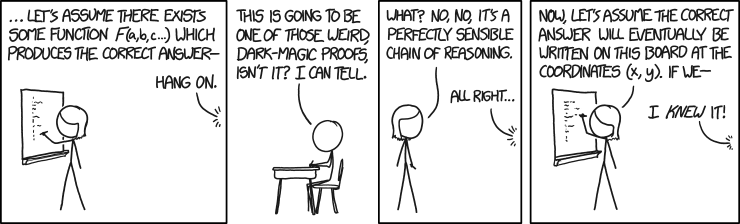
\includegraphics[scale=0.6]{xkcd_proofs.png}
    \caption{Comic from https://xkcd.wtf/1724/}
\end{figure}

\begin{example}[Classic]
Let $a, b$ be integers. We say that an integer is \textit{tasty} if it is expressible in the form $a^2+ab+b^2$. Prove that 2 is not tasty.
\end{example}
Classically, $a^2+ab+b^2$ is a so-called quadratic form. This suggests a direct proof is not feasible: enter the realm of contradictions.

\begin{proof}
We first suppose for the sake of contradiction that $2$ is expressible in this form. Then we have, for some $a,b$: 
$$a^2+ab+b^2=2 \implies (2a+b)^2+3b^2=8.$$

Now, the problem falls to simple casework: neither $b^2=0$, $b^2=1$ nor $b^2=4$ is possible, but we assumed initially that $2$ is tasty! Since a wrong assumption resulted in an absurd conclusion, this means that our initial assumption must be wrong. In other words, $2$ is not tasty.
\end{proof}

Another classical example is on the irrationality of $\sqrt{2}$. 
\begin{example}[Classic]
    Prove that $\sqrt{2}$ is irrational.
\end{example}
\begin{proof}
As again, we suppose on the contrary that $\sqrt{2}$ is rational, so $\sqrt{2}=\frac{m}{n}$ where $\gcd(m,n)=1$ (this just means that $\sqrt{2}$ can be expressed as a fraction in simplest terms).

Squaring, $$2=\frac{m^2}{n^2} \implies 2n^2=m^2.$$ Hence, $2|m \implies 4|m^2$ and so $2|n^2$. However, this is a contradiction because we initially defined $\gcd(m,n)=1$! 

This means that our initial assumption that $\sqrt{2}$ is rational was wrong. In other words, $\sqrt{2}$ is irrational.
\end{proof}
\subsubsection{Induction}
Formally, for a proposition $P(n)$, $n\in\mathbb{Z}^+$, if $P(1)$ is true and $P(k)$ is true $\implies$ $P(k+1)$ is true for some $k$ $\in\mathbb{Z}^+$, then $P(n)$ is true $\forall$ $n\in\mathbb{Z}^+$.
\begin{figure}[H]
    \centering
    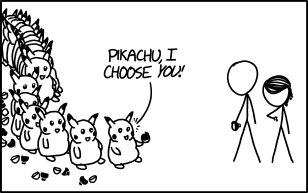
\includegraphics[scale=0.5]{xkcd_win_by_induction.png}
    \caption{Comic from https://xkcd.wtf/1516 - Win by Induction}
\end{figure}
Intuitively, this can be think of as a chain effect in a dominoes setup: if an arbitrary proposition being true implies the succeeding tile proposition is true, then the corresponding tile topples its succeeding tile, which in turn topples the next tile, and so on - except we have infinitely many domino tiles.

All of these toppling, however, is subject to a condition: the base case must be true. That is, the first tile must be knocked over for this chain effect of tiles toppling over each other to start. This is the so-called \textit{base case}.

Suppose we wish to prove that the proposition $P(n)$ is true for all $n$ $\in\mathbb{Z}^+$. 
\begin{proposition}
    A textbook induction proof follows this structure.
\begin{enumerate}
    \item \textbf{Base case}: Establish that $P(1)$ is true.
    \item \textbf{Inductive hypothesis/assumption}: Suppose that $P(k)$ is true for some arbitrary $k$ $\in\mathbb{Z}^+$. 
    \item \textbf{Inductive step}: Prove that $P(k)$ being true implies $P(k+1)$ is true. 
    \item \textbf{Conclude}: Since $P(1)$ is true and $P(k)$ being true implies $P(k+1)$ is true, then $P(n)$ is true for all $n$ (this is called the Principle of Mathematical Induction).
\end{enumerate}
\end{proposition}
This structure holds for most cases, although care must be taken in establishing the base case. If the given proposition holds over a different domain, say $n\geq 2$ instead of $n\geq 1$, then the base case will be $P(2)$ instead of $P(1)$.

Let us now showcase some applications of the induction technique. In general, most textbook proofs by induction do not follow this strict structure and merely outline the inductive step. For starters, we shall follow closely the structure given above.
\begin{example}[Classic]
    Prove that $1+2+\cdots+n=\frac{n(n+1)}{2}$ for all $n\in\mathbb{Z}^+$.
\end{example}
\begin{proof}
    Let $P(n)$ denote the proposition that $1+2+\cdots+n=\frac{n(n+1)}{2}$ for $n\in\mathbb{Z}^+$.

    \begin{enumerate}
        \item \textbf{Base case}: LHS of $P(1)$=1 and $RHS$ of $P(1)=\frac{1(1+1)}{2}=1$, so $P(1)$ is true.
        \item \textbf{Inductive hypothesis}: Suppose that $P(k)$ is true for some $k\geq 0$. That is, assume that $$1+2+\cdots+k=\frac{k(k+1)}{2}$$.
        \item \textbf{Inductive step}: To prove $P(k+1)$ is true, we begin with the LHS. This is because we can easily make use of the inductive hypothesis (keep an eye out for whenever you can use it!)
        \begin{align*}
            1+2+\cdots+k+(k+1) &= \frac{k(k+1)}{2}+(k+1) &\text{by inductive hypothesis} \\
            &=\frac{(k+1)(k+2)}{2} =\text{RHS of $P(k+1)$.}
        \end{align*} 
    \end{enumerate}
\end{proof}
\begin{example}[Classic]
    Prove that, for all integers $n \geq 0$ and real $x$, $|\sin{nx}|\leq n|\sin{x}|$.
\end{example}
\begin{proof}
    Let $P(n)$ denote the proposition that $|\sin{nx|}\leq n|\sin{x}|$ for integers $n\geq 0$. Note that now, the base case is $n=0$ instead of $n=1$!

    \begin{enumerate}
        \item \textbf{Base case}: LHS of $P(0)=0$ and $RHS$ of $P(0)=0\sin{0\cdot x}=0$, so $P(1)$ is true.
        \item \textbf{Inductive hypothesis}: Suppose that $P(k)$ is true for some $k \geq 0$. That is, assume that $$|\sin{kx}|\leq k|\sin{x}|$$.
        \item \textbf{Inductive step}: To prove $P(k+1)$ is true, we again begin with the LHS.
        \begin{align*}
            |\sin{(k+1)x}| &= |\sin{kx}\cos{x}+\cos{kx}\sin{x}| \\
            &\leq |\sin{kx}\cos{x}|+|\cos{kx}\sin{x}| &\text{by triangle inequality}\\
            &=|\sin{kx}||\cos{x}|+|\cos{kx}||\sin{x}| \\
            &\leq k|\sin{x}||\cos{x}|+|\cos{kx}||\sin{x}| &\text{by inductive hypothesis} \\
            &\leq k|\sin{x}|+|\sin{x}| \\
            &= (k+1)|\sin{x}|=\text{RHS of $P(k+1)$}
        \end{align*} 
    \end{enumerate}
\end{proof}
To end off the section on induction, we show an unorthodox way to finish the inductive step. It's not always the case that we can simply move from LHS to RHS.
\begin{example}[2021 H2 Further Math P1 Q4]
For real $x$ and any positive integer $n$, the function $F_n$ is defined by
    $$F_n(x)=\frac{x(x+1)(x+2)\cdots(x+n-1)}{n!}.$$
Prove by induction that, for all positive integers $n$, $F_n\left(\frac{1}{2}\right) < \frac{1}{\sqrt{2n+1}}$.
\end{example}
    The base case is simple, so we focus on the inductive assumption first. For the moment, write $x=\frac{1}{2}$ and assume that $F_k(x)<\frac{1}{\sqrt{2k+1}}$ (this is our inductive hypothesis!).
    
    We have
    \begin{align*}
        F_{k+1}(x)&=\frac{x(x+1)(x+2)\cdots(x+k-1)}{k!} \cdot \frac{x+k}{k+1} &\text{by inductive hypothesis}\\
        &< \frac{1}{\sqrt{2k+1}} \cdot \frac{2k+1}{2(k+1)} = \frac{2k+1}{2(k+1)\sqrt{2k+1}} \\
    \end{align*}
    How do we proceed? To start, we know that $\frac{2k+1}{2(k+1)} < 1$, but that gives $F_{k+1}(x) < \frac{1}{\sqrt{2k+1}}$, no good. On the other hand, our required form is $F_{k+1}(x) < \frac{1}{\sqrt{2k+3}}$, so the naive student may attempt to claim $\frac{1}{\sqrt{2k+1}} < \frac{1}{\sqrt{2k+3}}$, but this is not true!!
    
    To this end, we try the most obvious thing possible: we want $F_{k+1}(x) < \frac{1}{\sqrt{2k+3}}$, so it would be great if we have $\frac{2k+1}{2(k+1)\sqrt{2k+1}}<\frac{1}{\sqrt{2k+3}}$. Trying our luck:
    \begin{align*}
        \frac{2k+1}{2(k+1)\sqrt{2k+1}} < \frac{1}{\sqrt{2k+3}}
        &\Longleftrightarrow (2k+1)\sqrt{2k+3} < 2(k+1)\sqrt{2k+1} \\
        &\Longleftrightarrow (4k^2+4k+1)(2k+3) < (4k^2+8k+4)(2k+1) \\
        &\Longleftrightarrow 3(4k^2)+4k(2k+3)+(2k+3) < 4k^2+8k(2k+1)+4(2k+1) \\
        &\Longleftrightarrow 14k+3 < 16k+4 \Longleftrightarrow k > \frac{1}{2}
    \end{align*}
    Miraculously, our high power terms cancel off! Notice that we used "left-right" arrows instead of the usual "right" arrow. This "left-right" arrow indicates that the preceding line implies the next line, and the next line implies the preceding line. This means that our steps are \textbf{reversible}, so we can simply retrace our steps from the last line all the way back to the first line. This completes our induction proof, since the domain of our proposition is $k > 1$.

    The reader is encouraged to furnish a cleaned induction proof, unlike the one we have just shown. It is, however, the case that most induction proofs are found in this form, where only the inductive step is shown.
    \paragraph{Tangent: Central Binomial Coefficient}\label{algebra-cbc}
    We should probably be suspicious about why the cubic and quadratic terms in our inequalities cancel. Although, we should be equally suspicious about the choice of $x=\frac{1}{2}$. The function is defined for all real $x$, so why this specific rational number?
    
    We start by expanding $$F_n\left(\frac{1}{2}\right)=\frac{\frac{1}{2}\frac{3}{2}\frac{5}{2}\cdots\frac{2(n-1)+1}{2}}{n!}=\frac{1\cdot3\cdot5\cdots(2n-1)}{2^nn!}.$$
    Moreover, the product of the even integers: $2\cdot4\cdots2n=\frac{(2n)!}{2^n}$, so $$F_n\left(\frac{1}{2}\right)=\frac{1}{2^{2n}}\frac{(2n)!}{n!n!}=\frac{1}{2^{2n}}\binom{2n}{n}.$$
    
    As it turns out, $\binom{2n}{n}$ is the so-called \textbf{central binomial coefficient} (why?).
    
    The bound in the question asserts that $\binom{2n}{n} < \frac{4^n}{\sqrt{2n+1}}$, however Erdos argues that the best (asymptotic) bound is $\binom{2n}{n} < \frac{4^n}{\sqrt{\pi n}}$, as we will derive.
    
    The binomial coefficient arises in binomial expansions, so we shall consider a suitable one. For this, we look to the related binomial expansion for cosine. In particular, letting $z=e^{it}$, we have $\cos{t} = \frac{1}{2}\left(z+\frac{1}{z}\right)$, and \begin{align*}
        \cos^{2n} t &= \frac{1}{2^{2n}}\sum_{k=0}^{2n} \binom{2n}{k}z^{2n-2k} \\
        &= \frac{1}{2^{2n}}\sum_{k=0}^{2n} \binom{2n}{k}\cos{(2n-2k)t}+\frac{i}{2^{2n}}\sum_{k=0}^2n \binom{2n}{k}\sin{(2n-2k)t}
    \end{align*}
    Note that since $\cos^{2n}{t}$ is real, the imaginary part vanishes. Moreover, $$\binom{2n}{k}\cos{(2n-2k)t}+\binom{2n}{2n-k}\cos{(2k-2n)t}=2\binom{2n}{k}\cos{(2n-2k)t}\text{ by symmetry}.$$
    Hence,
    \begin{align*}
        \cos^{2n} t &= \frac{1}{2^{2n}}\sum_{k=0}^{2n} \binom{2n}{k}z^{2n-2k} \\
        &= \frac{1}{2^{2n}}\sum_{k=0}^{2n} \binom{2n}{k}\cos{(2n-2k)t}+\frac{i}{2^{2n}}\sum_{k=0}^{2n} \binom{2n}{k}\sin{(2n-2k)t} && \text{by de Moivre's theorem}\\
        &= \frac{1}{2^{2n}}\sum_{k=0}^{2n} \binom{2n}{k}\cos{(2n-2k)t} \\
        &= \frac{1}{2^{2n}}\left(\binom{2n}{n}+2\sum_{k=1}^{n-1}\binom{2n}{k}\cos{(2n-2k)t}\right)
    \end{align*}
    The substitution $j=n-k$ gives
    $$
        \cos^{2n} t = \frac{1}{2^{2n}}\left(\binom{2n}{n}+2\sum_{j=1}^{n}\binom{2n}{n-j}\cos{2jt}\right)
    \implies
        \int_{-\frac{\pi}{2}}^{\frac{\pi}{2}}\cos^{2n} t \,dt = \frac{\pi}{2^{2n}}\binom{2n}{n}.
    $$
    Thus, we have the chain of bounds:
    \begin{align}
        \binom{2n}{n}&=\frac{4^n}{\pi}\int_{-\frac{\pi}{2}}^{\frac{\pi}{2}}\cos^{2n}{x} \,dx < \frac{4^n}{\pi}\int_{-\frac{\pi}{2}}^{\frac{\pi}{2}}e^{-nx^2} \,dx \label{5.1-tangent-ineq}\\
        &< \frac{4^n}{\pi}\int_{-\infty}^{\infty}e^{-nx^2} \,dx = \frac{4^n}{\sqrt{\pi n}} \label{5.1-tangent-eq}
    \end{align}
\end{document}